\documentclass[main.tex]{subfiles}
\begin{document}


\chapter{Prototyp}
Um herauszufinden, welche der OSRE am leistungsstärksten ist, wurden drei Prototypen erstellt. Mit diesen soll erforscht werden, wie sich eine Applikation beim Einsatz der verschiedenen ORSE verhält. Es wurde darauf geachtet, dass der Prototyp nur genau die Komponenten besitzt, die für die Aufgabe benötigt werden.  

Jeder Prototyp ist zweiteilig. Die Prototypen besitzen die gleiche REST-Schnittstelle, welche die Anfragen entgegennimmt. Die REST-Schnittstelle leitet diese Anfrage an die entsprechenden Implementationen weiter. Dort werden diese Anfragen in konkrete PDFs umgesetzt. Im Folgenden werden die grundlegenden Aspekte der Implementationen näher betrachtet. 

\begin{reference}{Prototyp}
 Der Prototyp kann unter \url{https://github.com/denisbittante/DINF-BT-K/tree/master/3_Prototyp/Prototyp} gefunden werden.
\end{reference}

\section{Schnittstelle}


Die Schnittstelle wurde so implementiert, dass eine HTTP-POST-Anfrage entgegengenommen werden kann. Der Request-Body wird dem Interface '\texttt{PdfEngine}' weitergegeben. Dieses Interface wurde mithilfe der Spring-Annotation @Autowired eingesetzt. Damit besteht eine lose Koppelung der \acrshort{pdf}-Implementation und der Schnittstelle gegen aussen. Dank dieser Aufstellung kann nun einfach eine beliebige Implementation aufgerufen werden.

Die \acrshort{rest}-Schnittstelle bietet die drei PDF-Szenarien über die Endpunkte \texttt{/scenario1}, \texttt{/scenario2} und \texttt{/scenario3} an.   

\begin{lstlisting}[language=Java,caption={Auszug REST-Implementation },captionpos=b]

@RestController("/")
public class PdfServiceController {

	@Autowired
	private PdfEngine engine;

	@RequestMapping(method = RequestMethod.POST, path = "scenario1")
	public @ResponseBody PdfResponse scenario1(@RequestBody PdfRequestScenario1 req) {
		return engine.createPdfSzenario1(req);
	}
      ...
      
     // weitere  Endpunkte 
    
}
\end{lstlisting}

\subsection{Requests}
Die Endpunkte werden mit den folgenden POST-Bodys angesprochen. 


\subsubsection{Szenario 1}
Das JSON für das erste Szenario bildet das Modell für eine Aktivität ab. Diese soll einen Titel und eine Zeitangabe besitzen, wann diese stattfindet. Es wurden verschiedene Informationen hinterlegt, die für eine Freizeitbeschäftigung interessant wären, wie: Wer organisiert und welche Freunde oder Helfer werden eingeladen? Wo soll es stattfinden?  
\begin{lstlisting}[language=json,caption={JSON - Szenario 1},captionpos=b]
{"data": [
      {
      "title":          "Sommer-Fest",
      "datumVon":       "12.02.2017 16:00",
      "datumBis":       "12.02.2017 23:00",
      "description":    "Bringt Essen und gute Laune mit",
      "place":          "Musterstrasse 12\n888 Musterstadt\nSchweiz",
      "incharge":       "Denis Bittante",
      "helper":         "Lars Hauser, Max Muster",
      "author":         "Denis Bittante"
   }, ...
]}


\end{lstlisting}


\subsubsection{Szenario 2}
Szenario 2 ist sozusagen eine Zusammenfassung oder das Programm der interessanten Aktivitäten, die an einem Tag anstehen werden. Die Daten fassen die Eckdaten einer Aktivität zusammen, wie der Organisator und die Zeitangaben. Es gibt keine Details, aber eine Möglichkeit eine Fussnote zu versehen, die nach jedem Tag erscheinen soll. 
\begin{lstlisting}[language=json, caption={JSON - Szenario 2},captionpos=b]
{"group": [
      {
      "title":  "21.2.12 Vortraege fuer diesen Tag",
      "entries":[ {
            "time":         "19:00",
            "title":        "Ein Titel",
            "person":       "D.Bittante",
            "isSubtitle":   false
         },  ...
      ],
      "footer": "Special Information as Footnote"
   }, ...
      ]}


\end{lstlisting}


\subsubsection{Szenario 3}

Im dritten Szenario wurde entschieden, eine Kontaktliste zu erstellen, damit die Helfer und Freunde auch ausgedruckt werden können. Im Hinblick darauf, wie die Bilder und Tabellen eingefügt werden können, wurde hier entschieden, die Personendaten wie Vorname, Familienname und Adress- und Kontaktdaten zu hinterlegen, aber auch die Information zum Geschlecht. Dabei steht ’m’ für männlich (male) und ’f’ für female. Die Gender-Information soll dann auf der Kontaktliste als Gender-Symbol dargestellt werden.

\begin{lstlisting}[language=json,caption={JSON - Szenario 3},captionpos=b]
{"contacts": [
      {
      "gender":     "m",
      "name":       "Mustername",
      "firstname":  "Max",
      "address":    "Musterstrasse 12",
      "zip":        "9000",
      "place":      "Ort",
      "tel":        "+41 55 555 55 55",
      "mob":        "+41 55 555 55 55",
      "birthday":   "2.2.1988",
      "note":       "schlaue Notiz fuer diese Person",
      "email":      "max.muster2000@gmx.ch"
   }, ...
]}


\end{lstlisting}

\begin{reference}{JSON Request}
 Vollständige Request können unter \url{https://github.com/denisbittante/DINF-BT-K/tree/master/3_Prototyp/JSON_Request} gefunden werden.
\end{reference}
 


\subsection{Responses}
Die Responses der REST-Schnittstelle wurden einfach gehalten, daher werden die OSRE und das Szenario angegeben und im Feld \texttt{Status}, ob die Verarbeitung korrekt abgeschlossen wurde. Das generierte PDF ist als base64 encodiert und als Feld \texttt{file} in der Response zu finden. 
\begin{lstlisting}[language=json,caption={JSON - Antwort},captionpos=b]
{
   "name": "ApachePdfBox",
   "description": "Szenario 1",
   "file": "JVBERi0xLjQKJfb ... hyZWYKMTc2NAolJUVPRgo=",
   "status": "ok"
}

\end{lstlisting}




\section{Implementation}

Beim Einsetzen des Interfaces PDFEngine werden je nach Build eine der drei Implementationen instanziert (siehe Abbildung \ref{figure:pdfEngineImpl}). Jede dieser Klassen hat alle drei Szenarien zu implementieren.  


\begin{figure}[h]
 
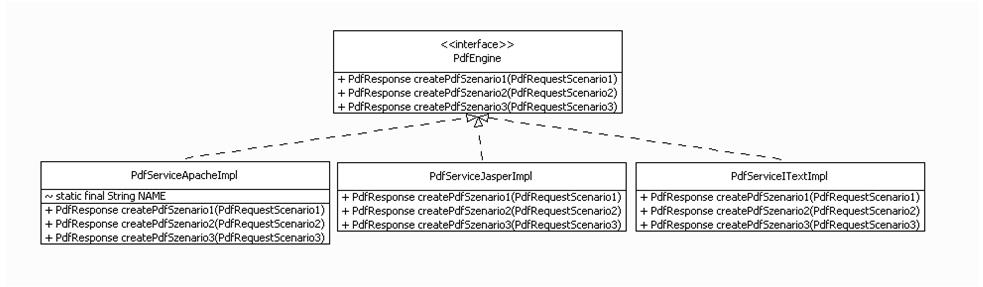
\includegraphics[width=\textwidth ]{pic/uml/PdfEngineImplemntierung.jpg}
 \caption{UML PDFEngine Implementierungen}
 \label{figure:pdfEngineImpl}
\end{figure}

Die einzelnen Szenarien wurden ebenfalls als Interfaces deklariert, damit jedes dieser Szenarios nicht anders oder nur teilweise implementiert wird. Als Basis-Klasse wurde die \texttt{AbstractScenario}-Klasse implementiert. Diese regelt den Aufbau, wie die temporären Files auf dem System abgelegt werden und wie diese wieder abgeräumt werden. Diese abstrakte Klasse übernimmt ebenfalls den Aufbau und das Handling des \texttt{PdfRequest} als Modell. Dieses Modell steht jeder Implementation über die Methode \texttt{getModel} im \texttt{AbstractSzenario} zur Verfügung (siehe Abbildung \ref{figure:szenImpl}).   

\begin{figure}[h]
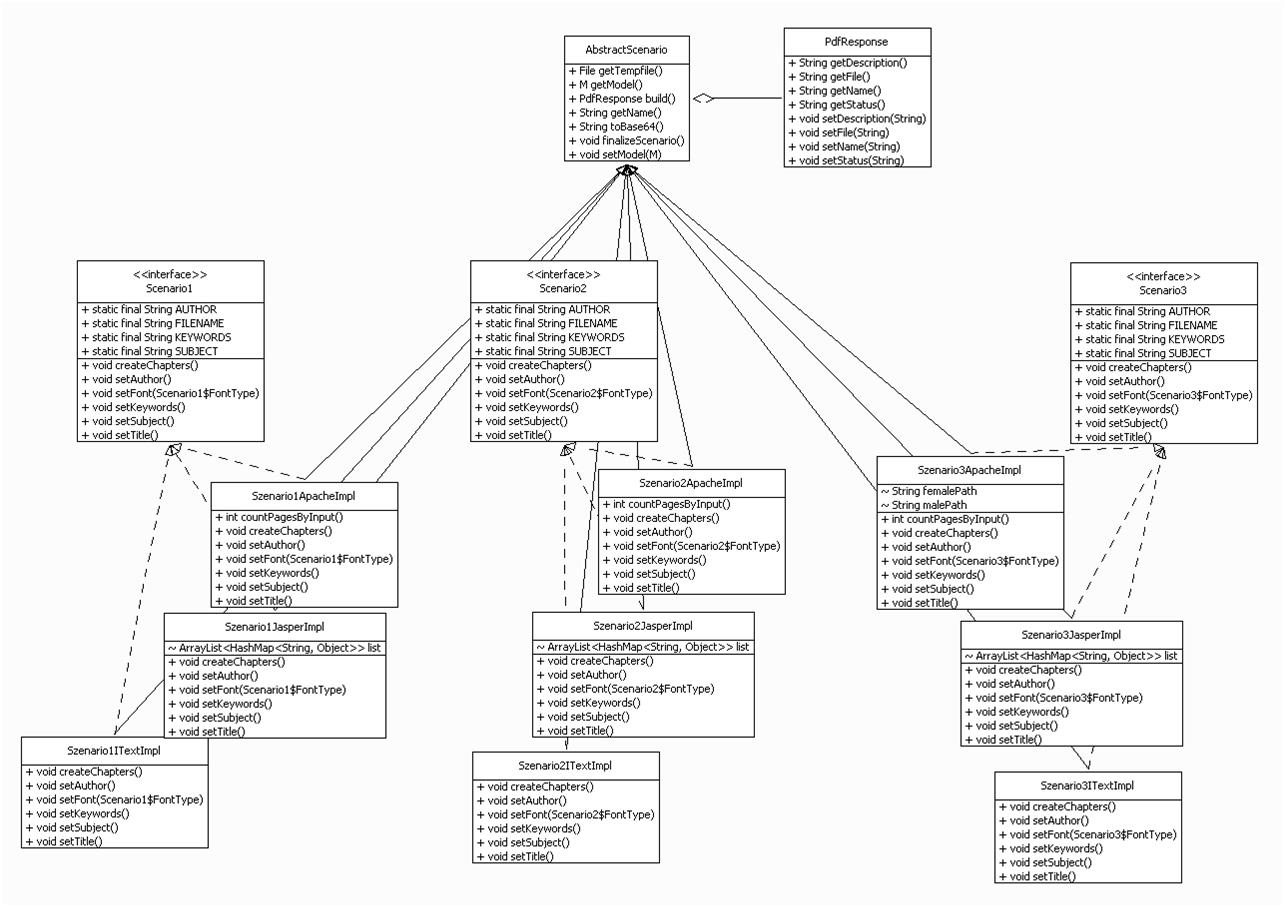
\includegraphics[width=\textwidth ]{pic/uml/SzenarioImplementation.jpg}
 \caption{UML Szenario Implementierungen}
 \label{figure:szenImpl}
\end{figure}


Die Implementationen sind sehr unterschiedlich aufgebaut denn z.B. muss für Apache PDFBox der Zeilenumbruch für einen langen Text selber entwickelt werden,  gleiches gilt für die Seitenumbrüche. Da es an  ein High-Level API fehlt, wurden keine Templates erstellt, wie es  JasperReports möglich macht. Da diese Layouts immer auf der Basis von spezifischen Daten-Inputs basieren, kann ein Flow-Pattern nicht implementiert werden. Apache PDF bietet sich an, um pixelgenaue Layouts zu erstellen, da die Texte mit Offset-Angaben ausgerichtet werden können.

Das API von iTest ist hingegen umfangreicher und klarer, z.B. werden Seiten automatisch neu generiert. Es benötigt keine Seitenangaben wie Rand und Grösse, da Standards diese bereits vorgeben.  Die Positionierung einzelner Elemente kann über die Canvas-Funktionen ebenfalls erreicht werden, z.B. beim Definieren von Footer oder Header. iText lässt auch eine dokumentenübergreifende Fonteinstellung definieren.

JasperReport nutzt die Templates, die im Programmcode mitgeliefert werden und kann somit mit wenig Implementation viele Anforderungen erfüllen. 


\subsection{Build / Deployment}

Die einzelnen JARs mit den gewünschten Implementationen können mittels Maven gebildet werden. Dazu wurde für jedes Produkt ein Profil eingerichtet. Dafür muss das Projekt vollständig gebildet werden, damit die einzelnen Implementationen als Archiv im Maven Repository erreichbar sind, und anschliessend kann der REST-Service gebildet und gestartet werden.  

\begin{lstlisting}[language=command.com,caption={CLI Installationskommandos},captionpos=b]


REM Bildet alle Maven Module 
cd ../dinf/app/ 
mvn clean install 

REM  Bildet den RestService mit gewuenschter OSRE Implementation     
cd ../dinf/app/rest-springboot/

mvn clean install -Pitext
REM (oder)
mvn clean install -Pjasper
REM (oder)
mvn clean install -Ppdfbox
\end{lstlisting}


Das generierte JAR kann über das heroku-Komamndo ebenfalls über die Konsole deployed werden. Da der Stand des gewünschten Dynos meist nicht bekannt ist, wurde nach dem Deployment auch der Dyno neu gestartet. 

\begin{lstlisting}[language=command.com,caption={CLI Deploymentkommandos},captionpos=b]

REM Deployed hier denn service mit der pdfbox implementation auf den Dyno 'dinf-app'
heroku deploy:jar  target\rest-service-pdfbox.jar --app dinf-app

REM Startet den Dyno namens 'dinf-app' erneut
heroku restart --app dinf-app



\end{lstlisting}

\subsection{Technische Details}
Um die Resultate dieses Experiments zu reproduzieren, sind folgende Eckdaten und Versionen nötig (siehe Tabelle \ref{softversion}). 


\begin{table}[!ht]
\centering
\begin{tabular}{ll}
Software          & Version   \\ \hline
Java        &      jdk 1.8.0.112      \\
Spring Boot &         1.5.8.RELEASE        \\

iText        &        7.1.0  \\
Apache PDFBox - Core &  2.0.1 \\
Apache PDFBox - fontbox & 2.0.0 \\
Apache PDFBox - jempbox & 1.8.11 \\
Apache PDFBox - xmpbox & 2.0.0 \\
Apache PDFBox - preflight & 2.0.0 \\
Apache PDFBox - pdfbox-tools & 2.0.0 \\
JasperReport & 6.4.3 \\
JasperReport - fonts & 4.0.0 \\
Maven   &  3.3.9 \\
 & \\


\end{tabular}
\caption{Prototyp Versionsangaben}
\label{softversion}

\end{table}
Der Stand von Heroku war zum Zeitpunkt der Tests wie folgt konfiguriert (siehe Tabelle \ref{herokuversion}).
\begin{table}[!hb]
\centering

\begin{tabular}{ll}

Heroku (PaaS)    & \\ \hline
Region & USA \\
Stack & heroku-16 \\
 & Ruby: 2.2, 2.3 und 2.4\\
 & OpenJDK: 7, 8, 9\\
 & PHP: 5.6, 7.0, 7.1\\
 & Python: 2.7, 3.5, 3.6\\
 & Go: Alle Versionen\\
 & Node: Alle Versionen \\
Buildpacks & heroku/jvm \\
Dyno Type & Standard-2X \\
RAM & 1GB \\
Anzahl Dyno & 1 \\


\end{tabular}
\caption{Heroku Konfiguration}
\label{herokuversion}
\end{table}




\end{document}
